\documentclass[11pt,a4paper]{article}

% ---------------------------------------------------------------
% Packages
% ---------------------------------------------------------------
\usepackage[T1]{fontenc}
\usepackage{amsmath, amsthm, mathtools}
\usepackage{libertinus}
\usepackage{libertinust1math}
\usepackage{bm}
\usepackage{graphicx}
\usepackage{xcolor}
\usepackage{tikz}
\usetikzlibrary{arrows.meta, patterns, decorations.pathmorphing}
\usepackage[most]{tcolorbox}
\usepackage{siunitx}
\sisetup{group-separator={\,}, group-minimum-digits=4, exponent-product=\cdot}
\usepackage{booktabs}
\usepackage{tabularx}
\usepackage[numbers,sort&compress]{natbib}
\usepackage{microtype}
\usepackage{parskip}
\usepackage[margin=2.5cm, headheight=20pt]{geometry}
\usepackage{titlesec}
\usepackage{fancyhdr}
\usepackage{lastpage}
\usepackage{hyperref}
\usepackage[capitalise,noabbrev]{cleveref}

\numberwithin{equation}{section}

% ---------------------------------------------------------------
% Corporate colours (sampled from the FAU logo) and layout
% ---------------------------------------------------------------
\definecolor{faublue}{RGB}{0,47,108}
\definecolor{fautech}{RGB}{119,159,181}

\hypersetup{colorlinks=true, linkcolor=faublue, citecolor=faublue, urlcolor=faublue,
  pdftitle={Solid Mechanics and Linear Finite Element Analysis}, pdfauthor={Ali Ghelichkhani}}

\titleformat{\section}{\sffamily\Large\bfseries\color{faublue}}{\thesection}{0.75em}{}
\titleformat{\subsection}{\sffamily\large\bfseries\color{faublue}}{\thesubsection}{0.7em}{}
\titleformat{\paragraph}[runin]{\sffamily\bfseries\color{faublue}}{}{0pt}{}
\titlespacing*{\paragraph}{0pt}{1.2ex plus 0.4ex}{0.6em}

\pagestyle{fancy}
\fancyhf{}
\fancyhead[L]{\sffamily\small\color{fautech}Materials Simulation Practical~2 \textbullet{} Part~I}
\fancyhead[R]{\raisebox{-0.2\height}{
\includegraphics[height=0.42cm]{figures/ww8.png}}}
\fancyfoot[L]{\sffamily\small\color{fautech}A.~Ghelichkhani}
\fancyfoot[R]{\sffamily\small\color{fautech}\thepage\ / \pageref*{LastPage}}
\renewcommand{\headrule}{\hbox to\headwidth{\color{fautech}\leaders\hrule height 0.4pt\hfill}}

% Task statements of the tutorial script (paraphrased); the box never separates from the
% heading above it, because "before" allows no page break
\newtcolorbox{task}[1]{enhanced, sharp corners, frame hidden,
  colback=fautech!12, borderline west={2.5pt}{0pt}{faublue},
  left=9pt, right=9pt, top=6pt, bottom=6pt, after skip=12pt,
  before={\par\nopagebreak\vskip 6pt},
  fontupper=\sffamily\small,
  before upper={{\bfseries\color{faublue}Task~#1.}\enspace}}
\setcounter{MaxMatrixCols}{20}

\theoremstyle{remark}
\newtheorem{remark}{Remark}[section]

% ---------------------------------------------------------------
% Notation
% ---------------------------------------------------------------
\newcommand{\R}{\mathbb{R}}
\newcommand{\grad}{\nabla}
\newcommand{\dv}{\operatorname{div}}
\newcommand{\bigO}[1]{\mathcal{O}\!\left(#1\right)}
\newcommand{\bu}{\bm{u}}
\newcommand{\bx}{\bm{x}}
\newcommand{\bX}{\bm{X}}
\newcommand{\bt}{\bm{t}}
\newcommand{\bn}{\bm{n}}
\newcommand{\bb}{\bm{b}}
\newcommand{\bv}{\bm{v}}
\newcommand{\bsig}{\bm{\sigma}}
\newcommand{\beps}{\bm{\varepsilon}}
\newcommand{\CC}{\mathbb{C}}
\newcommand{\bN}{\bm{N}}
\newcommand{\bB}{\bm{B}}
\newcommand{\bK}{\bm{K}}
\newcommand{\bP}{\bm{P}}
\newcommand{\bR}{\bm{R}}
\newcommand{\bd}{\bm{d}}
\newcommand{\bff}{\bm{f}}
\newcommand{\buh}{\hat{\bm{u}}}

\definecolor{cu}{RGB}{0,114,178}
\definecolor{cs}{RGB}{213,94,0}

\begin{document}

% ===============================================================
% Title page
% ===============================================================
\begin{titlepage}
  \noindent
  
\includegraphics[height=2.0cm]{figures/fau-techfak.png}\hfill
  \raisebox{0.6cm}{
\includegraphics[height=1.1cm]{figures/ww8.png}}

  \vspace{0.2cm}
  {\color{fautech}\rule{\textwidth}{0.6pt}}\\[0.1cm]
  {\sffamily\small\color{fautech}Institute of Materials Simulation (WW8)\hfill
    Winter semester 2026/27}

  \vspace*{3.4cm}
  {\sffamily\large\color{fautech}\textls[120]{MATERIALS SIMULATION PRACTICAL 2}\par}
  \vspace{0.5cm}
  {\sffamily\bfseries\color{faublue}\fontsize{30}{36}\selectfont
    Solid Mechanics and Linear\\[0.1em] Finite Element Analysis\par}
  \vspace{0.5cm}
  {\sffamily\Large\color{faublue}From the Balance of Momentum to a 1D Finite Element Code\par}
  \vspace{0.7cm}
  {\color{faublue}\rule{3cm}{2pt}}\par
  \vspace{0.4cm}
  {\sffamily\large Report, Part~I \textbullet{} Theory and Hand Calculations\par}

  \vfill
  {\sffamily
  \renewcommand{\arraystretch}{1.35}
  \begin{tabular}{@{}>{\small\color{fautech}}l@{\hspace{1.2em}}l@{}}
    Author     & Ali Ghelichkhani \\
    E-mail     & \href{mailto:ali.ghelichkhani@fau.de}{ali.ghelichkhani@fau.de} \\
    Supervisor & Yuxin Luo \\
    Module     & Foundations of Materials Simulation \\
    Institute  & Institute of Materials Simulation (WW8), FAU Erlangen-N\"urnberg \\
    Part~II    & Implementation, Jupyter notebook \texttt{fem1d.ipynb}
  \end{tabular}\par}
\end{titlepage}

% ===============================================================
% Abstract and contents
% ===============================================================
\section*{Abstract}
  We derive the governing equations of small-strain linear elasticity from the balance of
  linear momentum, specialize them to a clamped one-dimensional bar under tension, and
  develop the complete finite element machinery needed to solve that problem numerically.
  Balance of angular momentum and the existence of a strain energy density reduce the
  fourth-order stiffness tensor from $81$ to $36$ and finally to $21$ independent
  components. Multiplying the strong form by a test function and integrating by parts
  yields the weak form, whose solution needs to be only once differentiable. Linear
  Lagrange shape functions discretize the weak form element by element; the element
  integrals are evaluated with closed Newton--Cotes quadrature, for which we show that the
  $n$-point rule is exact for polynomials of degree $n-1$ and, for odd $n$, of degree $n$,
  so that two points already integrate the linear-element stiffness exactly. Assembly of
  the element matrices produces a singular, symmetric positive semi-definite, tridiagonal
  global stiffness matrix whose null space is the rigid-body translation; imposing one
  Dirichlet condition by a permutation of the global system removes that singularity. For
  one element we solve the resulting $2\times2$ system by hand and recover the analytical
  tip displacement $u(l) = Fl/(EA)$ exactly. The implementation, verification and the
  six-element analysis of Task~8.1 are reported in Part~II.

\tableofcontents
\clearpage

% ===============================================================
\section{Introduction}\label{sec:intro}
% ===============================================================

The mechanical response of a solid to external loading is governed by three ingredients
that are logically independent of one another: a \emph{kinematic} description that relates
displacements to strains, a \emph{balance law} that expresses the conservation of linear
and angular momentum, and a \emph{constitutive law} that connects stresses to strains and
encodes the material behaviour. Together they form a boundary value problem --- a partial
differential equation with boundary conditions --- that can be solved in closed form only
for a handful of idealized geometries.

The finite element method (FEM) is the standard numerical method for the elliptic partial
differential equations that result from elastostatics~\citep{zienkiewicz2013, hughes2000}.
Its central idea is to abandon the pointwise (\emph{strong}) form of the balance equation
in favour of an integral (\emph{weak}) form that holds only in an averaged sense against a
family of test functions. The weak form lowers the differentiability requirement on the
solution from two derivatives to one, and because an integral over a domain is the sum of
integrals over subdomains, it can be evaluated element by element on an arbitrary
partition of the body. Each element contributes a small, dense stiffness matrix; these are
assembled into a large sparse global system that is solved after boundary conditions have
been imposed.

In this report we follow that chain for the simplest non-trivial case, a straight elastic
bar of length $l$ clamped at $x = 0$ and loaded by a prescribed force $F$ at $x = l$. We
derive the local balance of momentum and its static form (\cref{sec:balance}), count the
independent components of the stiffness tensor and reduce the three-dimensional problem
to the one-dimensional bar equation (\cref{sec:constitutive}), construct the weak form
(\cref{sec:weak}), introduce linear shape functions and their derivatives
(\cref{sec:shape}), analyse the accuracy of closed Newton--Cotes quadrature
(\cref{sec:quadrature}), evaluate the element stiffness matrix and solve the one-element
problem by hand (\cref{sec:element}), assemble the global system and discuss its
properties (\cref{sec:assembly}), and impose Dirichlet conditions by a permutation of the
global system (\cref{sec:dirichlet}). \Cref{sec:results} summarizes the numerical results
of the six-element analysis. Each task of the tutorial script~\citep{script} is restated
in paraphrased form in a shaded box at the beginning of the section that answers it;
\cref{tab:taskmap} gives an overview and states where each task is treated.

\begin{table}[ht]
  \centering
  \caption{Correspondence between the tasks of the tutorial script and this report. Tasks
    marked ``Part~II'' are implementation tasks and are carried out in the accompanying
    Jupyter notebook \texttt{fem1d.ipynb}; the sections given for them discuss the
    underlying theory and the results.}
  \label{tab:taskmap}
  \begin{tabularx}{\linewidth}{lXl}
    \toprule
    Task & Content & Section \\
    \midrule
    1.1 & Static local balance of momentum; body forces & \ref{sec:statics} \\
    2.1 & Hooke's law in index notation; $81 \to 36$ components & \ref{sec:indexnotation} \\
    2.2 & Strain energy density and Schwarz's theorem; $36 \to 21$ & \ref{sec:21} \\
    2.3 & Reduction to the one-dimensional bar equation & \ref{sec:bar} \\
    3.1 & Weak form of the bar problem & \ref{sec:weakbar} \\
    4.1 & Linear shape functions; exactly representable functions & \ref{sec:shapefun} (+ Part~II) \\
    4.2 & Shape function derivatives $\bB$ & \ref{sec:bmatrix} (+ Part~II) \\
    5.1 & General quadrature routine & \ref{sec:quadrule} (+ Part~II) \\
    5.2 & Newton--Cotes schemes and their exactness & \ref{sec:exactness} (+ Part~II) \\
    5.3 & Element stiffness; one-element system solved by hand & \ref{sec:kelem}, \ref{sec:oneelement} \\
    6.1 & Equilibrium of the spring chain; global system & \ref{sec:spring} \\
    6.2 & Assembly routine & \ref{sec:assemblyroutine} (+ Part~II) \\
    6.3 & Properties of the global stiffness matrix & \ref{sec:properties} \\
    7.1 & Permutation matrix for a $4\times4$ system & \ref{sec:permutation} \\
    7.2 & General Dirichlet routine, non-zero values & \ref{sec:nonzero} (+ Part~II) \\
    8.1 & Six-element analysis and post-processing & \ref{sec:results} (+ Part~II) \\
    \bottomrule
  \end{tabularx}
\end{table}

% ===============================================================
\section{Kinematics and balance equations}\label{sec:balance}
% ===============================================================

\subsection{Kinematic measures}\label{sec:kinematics}

A material point of the body is labelled by its position $\bX$ in the stress-free
reference configuration $\mathcal{B}_0$ and occupies the position
$\bx = \bm{\chi}(\bX,t)$ in the current configuration $\mathcal{B}(t)$. The displacement
is the difference of the two,
\begin{equation}\label{eq:displacement}
  \bu(\bX,t) = \bm{\chi}(\bX,t) - \bX,
\end{equation}
and velocity and acceleration are its first and second material time derivatives,
$\bv = \dot{\bu}$ and $\bm{a} = \ddot{\bu}$. For small deformations, where the components
of the displacement gradient are small compared to unity, the strain measure is the
symmetric part of that gradient,
\begin{equation}\label{eq:strain}
  \beps(\bX,t) = \frac{1}{2}\left(
    \frac{\partial \bu}{\partial \bX} + \left(\frac{\partial \bu}{\partial \bX}\right)^{\mathsf{T}}
  \right),
  \qquad
  \varepsilon_{ij} = \frac{1}{2}\left(\partial_j u_i + \partial_i u_j\right).
\end{equation}
Taking the symmetric part removes the infinitesimal rotation, which is the skew part of
the gradient and produces no strain energy. By construction $\beps = \beps^{\mathsf{T}}$,
a property that we use repeatedly below.

\subsection{Local balance of linear momentum}\label{sec:localbalance}

Newton's second law states that the rate of change of the linear momentum $\bm{p}$ of a
body equals the net force $\bm{F}$ acting on it. For a continuum the momentum and the
force are integrals over the volume and the surface of the body,
\begin{equation}\label{eq:integralbalance}
  \bm{p} = \int_{\mathcal{B}} \rho\,\dot{\bu}\,\mathrm{d}V,
  \qquad
  \bm{F} = \int_{\partial\mathcal{B}} \bt\,\mathrm{d}A + \int_{\mathcal{B}} \rho\,\bb\,\mathrm{d}V,
\end{equation}
with the mass density $\rho$, the traction vector $\bt$ on the surface and the body force
density $\bb$ (force per unit mass). Cauchy's theorem expresses the traction on a cut with
outward normal $\bn$ through the stress tensor, $\bt = \bsig\cdot\bn$. Inserting this,
applying the divergence theorem to the surface integral and demanding that the resulting
volume integral vanish for every subbody gives the local form
\begin{equation}\label{eq:localbalance}
  \rho\,\ddot{\bu} = \dv\bsig + \rho\,\bb.
\end{equation}
The same argument applied to the balance of angular momentum yields the symmetry of the
Cauchy stress tensor,
\begin{equation}\label{eq:sigmasym}
  \bsig = \bsig^{\mathsf{T}},
\end{equation}
which reduces its nine components to six independent ones.

\subsection{The static case (Task 1.1)}\label{sec:statics}

\begin{task}{1.1}
  Simplify the local balance of linear momentum for the static case, in which the
  acceleration vanishes. Give an example of a body force other than gravity, and describe
  a situation in which body forces may be neglected.
\end{task}

In statics no material point accelerates, $\ddot{\bu} = \bm{0}$, and the left-hand side
of~\eqref{eq:localbalance} vanishes. What remains is the equilibrium equation
\begin{equation}\label{eq:equilibrium}
  \boxed{\;\dv\bsig + \rho\,\bb = \bm{0}.\;}
\end{equation}
Every material point is in equilibrium: the divergence of the stress field, which is the
net surface force per unit volume acting on an infinitesimal element, is balanced by the
body force acting on the same element.

\paragraph{Body forces other than gravity.}
A body force acts on the mass or charge distributed throughout the volume rather than on
the surface. Besides gravity, $\bb = \bm{g}$, the most common examples are:
\begin{itemize}\setlength{\itemsep}{1pt}
  \item \emph{Inertial (fictitious) forces in a non-inertial frame.} For a component
    rotating with angular velocity $\bm{\omega}$, writing the balance in the co-rotating
    frame introduces the centrifugal body force $\bb = -\bm{\omega}\times(\bm{\omega}\times\bx)$
    and the Coriolis force $\bb = -2\,\bm{\omega}\times\dot{\bu}$. This is how turbine
    blades and flywheels are analysed.
  \item \emph{Electromagnetic (Lorentz) forces.} In a conductor carrying the current
    density $\bm{j}$ in a magnetic flux density $\bm{B}$, the force per unit volume is
    $\bm{j}\times\bm{B}$. This drives electromagnetic forming and the loading of
    high-field magnet coils.
  \item \emph{Thermal and magnetostrictive ``forces''.} A non-uniform eigenstrain field,
    for example a thermal strain $\alpha\,\Delta T(\bx)\,\bm{I}$, can be moved to the
    right-hand side of~\eqref{eq:equilibrium} and then acts exactly like a body force.
\end{itemize}

\paragraph{When body forces may be neglected.}
Both terms in~\eqref{eq:equilibrium} have the dimension of stress per length. Over a
body of characteristic size $L$ carrying a characteristic stress $\sigma_0$, the surface
term scales as $\sigma_0/L$ and the body-force term as $\rho g$, so their ratio is
\begin{equation}\label{eq:ratio}
  \frac{\|\rho\,\bb\|}{\|\dv\bsig\|} \sim \frac{\rho g L}{\sigma_0}.
\end{equation}
For the bar of \cref{sec:bar}, with steel ($\rho \approx 7.85\;\mathrm{g/cm^3}$, $g = 9.81\;\mathrm{m/s^2}$), $L = 50\;\mathrm{mm}$ and
$\sigma_0 = F/A = 5\;\mathrm{N}/25\;\mathrm{mm^2} = 0.2\;\mathrm{N/mm^2}$, the ratio is
$\rho g L/\sigma_0 \approx 3.85\cdot10^{-6}/0.2 \approx 2\cdot10^{-5}$. Gravity is
therefore five orders of magnitude smaller than the applied load and is neglected, which
is what we do by setting $b = 0$ in Task~5.3. In general, body forces are negligible for
small, stiff, strongly loaded components, and they must be retained for large structures
under their own weight (dams, tall buildings), for rotating machinery, and whenever the
externally applied load is small.

% ===============================================================
\section{Constitutive equations}\label{sec:constitutive}
% ===============================================================

The kinematic relation~\eqref{eq:strain} and the balance law~\eqref{eq:equilibrium} hold
for every material, but they do not close the problem. In the isothermal case the unknowns
are the six components of $\bsig$, the three components of $\bu$ and the density, that is
thirteen fields, whereas the balance of linear momentum supplies three equations and the
balance of mass one. The missing equations are supplied by a constitutive law
$\bsig = f(\beps)$, which carries all the information about the material. The simplest
choice is a linear map, Hooke's law,
\begin{equation}\label{eq:hooke}
  \bsig = \CC : \beps.
\end{equation}

\subsection{Index notation and the first reduction (Task 2.1)}\label{sec:indexnotation}

\begin{task}{2.1}
  Write Hooke's law in index notation and state over which indices the Einstein summation
  convention applies. How many components does $\CC$ have in three dimensions? Show that
  the symmetry of the stress and strain tensors reduces the number of independent
  components to $36$.
\end{task}

The double contraction in~\eqref{eq:hooke} contracts the last two indices of the
fourth-order tensor with the two indices of the strain tensor, so that in index notation
\begin{equation}\label{eq:hooke-index}
  \boxed{\;\sigma_{ij} = C_{ijkl}\,\varepsilon_{kl},\;}
  \qquad i,j,k,l \in \{1,2,3\}.
\end{equation}
The summation convention applies to the repeated indices $k$ and $l$ only; each term is
therefore a sum of nine products. The indices $i$ and $j$ appear once on each side and are
free: \eqref{eq:hooke-index} is a set of nine scalar equations. In three dimensions each
of the four indices runs over three values, so in general
\begin{equation}\label{eq:81}
  \#\,C_{ijkl} = 3^4 = 81.
\end{equation}

Not all of these can be independent. Because $\bsig$ is symmetric,
$\sigma_{ij} = \sigma_{ji}$, the left-hand sides of the equations with index pairs $(ij)$
and $(ji)$ are equal for every admissible strain, and so the coefficients must agree,
\begin{equation}\label{eq:minor1}
  C_{ijkl} = C_{jikl}.
\end{equation}
Because $\beps$ is symmetric, $\varepsilon_{kl} = \varepsilon_{lk}$, the products
$C_{ijkl}\varepsilon_{kl}$ and $C_{ijlk}\varepsilon_{lk}$ enter the same sum and only the
symmetric part of $C$ in its last two indices is ever activated; we may therefore take it
symmetric without loss of generality,
\begin{equation}\label{eq:minor2}
  C_{ijkl} = C_{ijlk}.
\end{equation}
Relations~\eqref{eq:minor1} and~\eqref{eq:minor2} are called the \emph{minor symmetries}.
Each of them replaces an unordered pair of indices by a single composite index: the
symmetric pairs $(ij)$ are
\begin{equation*}
  (11),\;(22),\;(33),\;(12)=(21),\;(13)=(31),\;(23)=(32),
\end{equation*}
that is $\tfrac{1}{2}\cdot 3\cdot 4 = 6$ instead of $9$ possibilities, and the same holds
for $(kl)$. Hence
\begin{equation}\label{eq:36}
  \boxed{\;\#\,C_{ijkl} = 6\times 6 = 36.\;}
\end{equation}
This is the reason why Hooke's law can be written in the Voigt notation as a $6\times6$
matrix acting on the six-component stress and strain vectors.

\subsection{Strain energy density and the second reduction (Task 2.2)}\label{sec:21}

\begin{task}{2.2}
  Show that the stiffness tensor has only $21$ independent components if, in addition to
  the symmetries of Task~2.1, it is derived from a strain energy density
  $W = \tfrac{1}{2}\,\bsig:\beps$ through $\CC = \partial^2 W / \partial\beps\,\partial\beps$.
  (Hint: Schwarz's theorem.)
\end{task}

Assume the existence of a strain energy density $W(\beps)$, a potential whose derivative
with respect to the strain gives the stress. For the linear law~\eqref{eq:hooke} it is the
quadratic form
\begin{equation}\label{eq:W}
  W = \frac{1}{2}\,\bsig:\beps = \frac{1}{2}\,C_{ijkl}\,\varepsilon_{ij}\,\varepsilon_{kl},
\end{equation}
and the stiffness tensor is recovered as its second derivative,
\begin{equation}\label{eq:Cfrom W}
  C_{ijkl} = \frac{\partial^2 W}{\partial \varepsilon_{ij}\,\partial \varepsilon_{kl}}.
\end{equation}
Because $W$ is a twice continuously differentiable function of the strain components,
Schwarz's theorem states that mixed partial derivatives commute,
\begin{equation}\label{eq:schwarz}
  \frac{\partial^2 W}{\partial \varepsilon_{ij}\,\partial \varepsilon_{kl}}
  = \frac{\partial^2 W}{\partial \varepsilon_{kl}\,\partial \varepsilon_{ij}}
  \qquad\Longrightarrow\qquad
  C_{ijkl} = C_{klij}.
\end{equation}
This is the \emph{major symmetry}: the two composite indices $I = (ij)$ and $J = (kl)$ may
be exchanged. In the Voigt picture of \cref{sec:indexnotation}, the $6\times6$ matrix
$C_{IJ}$ is therefore symmetric, and a symmetric $n\times n$ matrix has
$n(n+1)/2$ independent entries. With $n = 6$,
\begin{equation}\label{eq:21}
  \boxed{\;\#\,C_{IJ} = \frac{6\cdot 7}{2} = 21.\;}
\end{equation}
Twenty-one constants describe the most general anisotropic linear elastic solid, the
triclinic crystal. Additional material symmetries reduce this number further: nine for
orthotropic, five for transversely isotropic, three for cubic, and finally two --- the
Lam\'e constants $\lambda$ and $\mu$ --- for isotropy, where
\begin{equation}\label{eq:isotropic}
  C_{ijkl} = \lambda\,\delta_{ij}\delta_{kl} + \mu\left(\delta_{ik}\delta_{jl} + \delta_{il}\delta_{jk}\right),
  \qquad
  E = \frac{\mu\,(3\lambda + 2\mu)}{\lambda + \mu},
  \qquad
  \nu = \frac{\lambda}{2(\lambda+\mu)}.
\end{equation}

\begin{remark}
  The major symmetry is not a kinematic identity but a statement about the material: it
  holds precisely for \emph{hyperelastic} materials, for which the stress derives from a
  potential and the work done on a closed strain cycle vanishes. A linear law with
  $C_{ijkl} \neq C_{klij}$ would be consistent with the balance laws but would create or
  destroy energy in a closed cycle, violating the second law of thermodynamics.
\end{remark}

\subsection{Reduction to the one-dimensional bar (Task 2.3)}\label{sec:bar}

\begin{task}{2.3}
  Consider a bar of length $l$, clamped at $x=0$ and statically loaded by a prescribed
  force $F$ at $x=l$. The material is isotropic and homogeneous with constant density; the
  cross-section $A$ does not change under load ($\nu = 0$). Show that the local balance of
  linear momentum reduces in one dimension to
  \begin{equation*}
    \frac{\mathrm{d}}{\mathrm{d}x}\!\left(EA\,\frac{\mathrm{d}u}{\mathrm{d}x}\right) + A\rho\,b(x) = 0.
  \end{equation*}
\end{task}

\begin{figure}[ht]
  \centering
  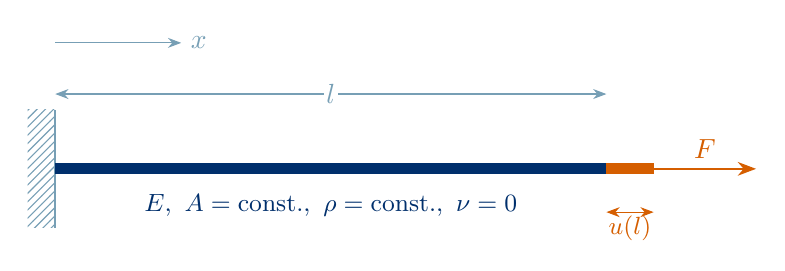
\begin{tikzpicture}[>=Stealth, scale=1.0]
    % wall
    \fill[pattern=north east lines, pattern color=fautech] (-0.35,-0.75) rectangle (0,0.75);
    \draw[fautech, thick] (0,-0.75) -- (0,0.75);
    % bar
    \draw[faublue, line width=4pt] (0,0) -- (7,0);
    \draw[cs, line width=4pt] (7,0) -- (7.6,0);
    % load
    \draw[->, cs, thick] (7.6,0) -- (8.9,0) node[above, midway] {$F$};
    % dimensions
    \draw[<->, fautech] (0,0.95) -- (7,0.95) node[midway, fill=white, inner sep=1pt] {$l$};
    \draw[<->, cs] (7,-0.55) -- (7.6,-0.55) node[midway, below, inner sep=1pt] {\small $u(l)$};
    \draw[->, fautech] (0,1.6) -- (1.6,1.6) node[right] {$x$};
    \node[faublue, below] at (3.5,-0.2) {\small $E,\ A = \text{const.},\ \rho = \text{const.},\ \nu = 0$};
  \end{tikzpicture}
  \caption{The clamped bar of Task~2.3 in the reference (blue) and the deformed
    configuration (orange). The displacement field $u(x)$ vanishes at the clamped end and
    reaches $u(l)$ at the loaded end.}
  \label{fig:bar}
\end{figure}

The geometry is shown in \cref{fig:bar}. The bar is slender, so the only non-vanishing
displacement component is the axial one and it depends on the axial coordinate alone,
\begin{equation}\label{eq:1dansatz}
  \bu = u(x)\,\bm{e}_1.
\end{equation}
With $\nu = 0$ the cross-section does not contract, so $u_2 = u_3 = 0$ exactly and no
lateral strain is generated. Inserting~\eqref{eq:1dansatz} into~\eqref{eq:strain} leaves a
single strain component,
\begin{equation}\label{eq:1dstrain}
  \varepsilon_{11} = \frac{\mathrm{d}u}{\mathrm{d}x} \eqqcolon \varepsilon(x),
  \qquad \text{all other } \varepsilon_{ij} = 0.
\end{equation}
For $\nu = 0$ the isotropic law~\eqref{eq:isotropic} gives $\lambda = 0$ and
$\mu = E/2$, so that $C_{1111} = \lambda + 2\mu = E$ and the lateral normal stresses
$\sigma_{22} = \sigma_{33} = \lambda\,\varepsilon_{11} = 0$ vanish. The only non-zero
stress component is therefore the uniaxial one,
\begin{equation}\label{eq:1dstress}
  \sigma(x) \coloneqq \sigma_{11} = E\,\varepsilon(x) = E\,\frac{\mathrm{d}u}{\mathrm{d}x}.
\end{equation}
The first component of the static balance~\eqref{eq:equilibrium} reads
$\partial_1\sigma_{11} + \partial_2\sigma_{12} + \partial_3\sigma_{13} + \rho b_1 = 0$;
the shear stresses vanish for the ansatz~\eqref{eq:1dansatz}, which leaves
\begin{equation}\label{eq:1dpointwise}
  \frac{\mathrm{d}\sigma}{\mathrm{d}x} + \rho\,b(x) = 0.
\end{equation}
This is a statement per unit volume. The one-dimensional model, however, describes the
bar by quantities integrated over the cross-section: the internal normal force
$N(x) = \sigma(x)A$ and the line load $A\rho b(x)$. Multiplying~\eqref{eq:1dpointwise} by
the cross-sectional area and using that $A$ does not depend on $x$ --- or, for a bar with
a slowly varying section, writing the equilibrium of the slice $[x, x+\mathrm{d}x]$
directly as $\mathrm{d}(\sigma A)/\mathrm{d}x + A\rho b = 0$ --- and inserting the
constitutive law~\eqref{eq:1dstress} gives
\begin{equation}\label{eq:barode}
  \boxed{\;\frac{\mathrm{d}}{\mathrm{d}x}\!\left(EA\,\frac{\mathrm{d}u}{\mathrm{d}x}\right)
    + A\rho\,b(x) = 0 \quad\text{in } (0,l),\;}
\end{equation}
which is the required result. Its boundary conditions are the Dirichlet condition at the
clamp and the Neumann condition at the loaded end,
\begin{equation}\label{eq:barbc}
  u(0) = 0,
  \qquad
  \sigma(l)\,A = EA\,\frac{\mathrm{d}u}{\mathrm{d}x}\bigg|_{x=l} = F.
\end{equation}
\Cref{eq:barode} is a second-order ordinary differential equation of the same elliptic
type as the Laplace equation of Practical~1; the Dirichlet condition fixes the otherwise
undetermined rigid-body translation. For constant $EA$ and $b = 0$ the solution is the
linear field
\begin{equation}\label{eq:analytic}
  u(x) = \frac{F\,x}{EA},
  \qquad
  \sigma(x) = \frac{F}{A} = \text{const.},
\end{equation}
which serves as the reference solution for all numerical results below.

% ===============================================================
\section{Weak form}\label{sec:weak}
% ===============================================================

\subsection{The weak form in three dimensions}\label{sec:weak3d}

The strong form~\eqref{eq:equilibrium} demands that the equilibrium hold at every single
material point, which requires $\bu$ to be twice continuously differentiable. The finite
element discretization uses piecewise polynomials whose derivatives jump across element
boundaries, so this requirement must be relaxed. To do so one multiplies the balance
equation by a test function $\delta\bu$ --- a virtual displacement, which must vanish on
the Dirichlet boundary $\Gamma_{\mathrm{u}}$ where $\bu$ is prescribed --- and integrates
over the body:
\begin{equation}\label{eq:weak-start}
  \int_{\mathcal{B}} \left(\dv\bsig\right)\cdot\delta\bu \,\mathrm{d}V
  + \int_{\mathcal{B}} \rho\,\bb\cdot\delta\bu \,\mathrm{d}V = 0.
\end{equation}
The product rule $\dv(\bsig\cdot\delta\bu) = (\dv\bsig)\cdot\delta\bu
+ \bsig^{\mathsf{T}} : \operatorname{grad}(\delta\bu)$ moves one derivative from the stress
onto the test function; the divergence theorem converts the remaining divergence into a
surface integral, on which $\delta\bu = \bm{0}$ on $\Gamma_{\mathrm{u}}$ and
$\bsig\cdot\bn = \bar{\bt}$ on the Neumann boundary $\Gamma_{\mathrm{t}}$. With Hooke's
law this gives the weak form
\begin{equation}\label{eq:weak3d}
  \int_{\mathcal{B}} \left(\CC:\beps\right) : \operatorname{grad}(\delta\bu)\,\mathrm{d}V
  = \int_{\mathcal{B}} \rho\,\bb\cdot\delta\bu\,\mathrm{d}V
  + \int_{\Gamma_{\mathrm{t}}} \bar{\bt}\cdot\delta\bu\,\mathrm{d}A .
\end{equation}
Only first derivatives of $\bu$ and $\delta\bu$ appear. Mechanically, \eqref{eq:weak3d} is
the principle of virtual work: the internal virtual work on the left equals the external
virtual work of the body and surface loads on the right.

\subsection{Weak form of the bar problem (Task 3.1)}\label{sec:weakbar}

\begin{task}{3.1}
  Show that the weak form of the bar problem~\eqref{eq:barode} is
  \begin{equation*}
    \int_0^l \frac{\mathrm{d}u}{\mathrm{d}x}\,EA\,\frac{\mathrm{d}\,\delta u}{\mathrm{d}x}\,\mathrm{d}x
    = \int_0^l A\rho\,b(x)\,\delta u(x)\,\mathrm{d}x + \underbrace{\bar{t}A}_{F}\,\delta u(l).
  \end{equation*}
\end{task}

We repeat the three steps of \cref{sec:weak3d} in one dimension. Let $\delta u$ be an
arbitrary test function that satisfies the homogeneous Dirichlet condition
$\delta u(0) = 0$ --- a virtual displacement must not violate the kinematic constraint at
the clamp. Multiplying~\eqref{eq:barode} by $\delta u$ and integrating over the bar gives
\begin{equation}\label{eq:weak1}
  \int_0^l \frac{\mathrm{d}}{\mathrm{d}x}\!\left(EA\,\frac{\mathrm{d}u}{\mathrm{d}x}\right)\delta u \,\mathrm{d}x
  + \int_0^l A\rho\,b\,\delta u \,\mathrm{d}x = 0.
\end{equation}
Integration by parts of the first integral --- the one-dimensional version of the product
rule together with the divergence theorem --- yields
\begin{equation}\label{eq:weak2}
  \int_0^l \frac{\mathrm{d}}{\mathrm{d}x}\!\left(EA\,\frac{\mathrm{d}u}{\mathrm{d}x}\right)\delta u \,\mathrm{d}x
  = \left[EA\,\frac{\mathrm{d}u}{\mathrm{d}x}\,\delta u\right]_0^l
  - \int_0^l EA\,\frac{\mathrm{d}u}{\mathrm{d}x}\,\frac{\mathrm{d}\,\delta u}{\mathrm{d}x}\,\mathrm{d}x .
\end{equation}
The boundary term is evaluated with the two boundary conditions~\eqref{eq:barbc}. At
$x = 0$ the test function vanishes, $\delta u(0) = 0$, so that end contributes nothing ---
this is exactly how a Dirichlet condition enters the weak form, implicitly through the
admissible test functions. At $x = l$ the bracket contains the prescribed Neumann data,
$EA\,u'(l) = \sigma(l)A = \bar{t}A = F$. Hence
\begin{equation}\label{eq:weak3}
  \left[EA\,\frac{\mathrm{d}u}{\mathrm{d}x}\,\delta u\right]_0^l = F\,\delta u(l).
\end{equation}
Substituting~\eqref{eq:weak2} and~\eqref{eq:weak3} into~\eqref{eq:weak1} and rearranging
gives the weak form of the bar problem,
\begin{equation}\label{eq:weakbar}
  \boxed{\;
  \int_0^l \frac{\mathrm{d}u}{\mathrm{d}x}\,EA\,\frac{\mathrm{d}\,\delta u}{\mathrm{d}x}\,\mathrm{d}x
  = \int_0^l A\rho\,b(x)\,\delta u \,\mathrm{d}x + F\,\delta u(l),
  \;}
\end{equation}
which is the required result. Two features are worth emphasizing. First, the Neumann
condition is \emph{natural}: it appears by itself in the right-hand side and no longer has
to be imposed on the solution space; in the discrete system it is simply an entry of the
load vector. Second, the Dirichlet condition is \emph{essential}: it must be built into
the function spaces for $u$ and $\delta u$ and, in the discrete system, has to be imposed
explicitly on the matrix (\cref{sec:dirichlet}).

% ===============================================================
\section{Discretization and shape functions}\label{sec:shape}
% ===============================================================

Because an integral over the bar is the sum of integrals over non-overlapping subintervals,
the weak form~\eqref{eq:weakbar} can be written as a sum over $n_{\mathrm{el}}$ elements
$e_k = [x_k, x_{k+1}]$,
\begin{equation}\label{eq:elementsum}
  \sum_{k=1}^{n_{\mathrm{el}}}\left\{
    \int_{e_k} \frac{\mathrm{d}u}{\mathrm{d}x}\,EA\,\frac{\mathrm{d}\,\delta u}{\mathrm{d}x}\,\mathrm{d}x
    - \int_{e_k} A\rho\,b\,\delta u\,\mathrm{d}x
    - \bar{t}_e A\,\delta u \big|_{\partial e_k}
  \right\} = 0 .
\end{equation}
Inside each element the unknown field is replaced by an interpolation of its nodal values.

\subsection{Linear Lagrange shape functions (Task 4.1)}\label{sec:shapefun}

\begin{task}{4.1}
  Sketch the six elements of the discretization and the two linear shape functions
  $N_1, N_2$ on each of them. Implement the shape functions for one element and test the
  approximation with three functions of your choice. Which of them are represented
  exactly? What does this imply for the displacement and stress fields on the element
  level?
\end{task}

The interpolation is built from Lagrange basis polynomials, which take the value one at
``their'' node and vanish at all others, $l_i(x_j) = \delta_{ij}$. On a two-node element
with nodes at $x_1^e$ and $x_2^e$ of length $h = x_2^e - x_1^e$ they are the two linear
functions
\begin{equation}\label{eq:shapefun}
  N_1(x) = \frac{x_2^e - x}{h},
  \qquad
  N_2(x) = \frac{x - x_1^e}{h},
  \qquad
  N_1(x) + N_2(x) = 1 .
\end{equation}
\Cref{fig:mesh} sketches the six-element mesh of Task~8.1 with the shape function pairs
drawn on each element. The interpolated displacement field and its vector form are
\begin{equation}\label{eq:interp}
  \tilde{u}(x) = \sum_{i=1}^{N_{\max}} N_i(x)\,\hat{u}_i
  = \underbrace{\begin{bmatrix} N_1(x) & N_2(x)\end{bmatrix}}_{\bN(x)}
    \begin{bmatrix} \hat{u}_1 \\ \hat{u}_2 \end{bmatrix}
  = \bN(x)\cdot\buh .
\end{equation}

\begin{figure}[ht]
  \centering
  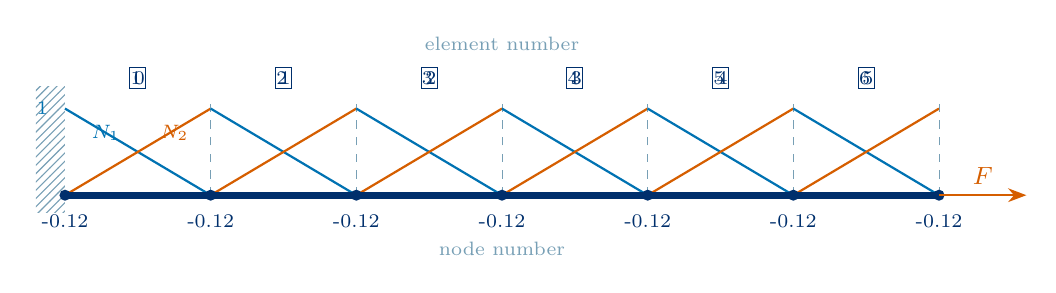
\begin{tikzpicture}[>=Stealth, x=1.85cm, y=1.1cm]
    % wall
    \fill[pattern=north east lines, pattern color=fautech] (-0.2,-0.2) rectangle (0,1.25);
    % shape functions
    \foreach \k in {0,...,5} {
      \draw[cu, thick] (\k,1) -- (\k+1,0);
      \draw[cs, thick] (\k,0) -- (\k+1,1);
      \draw[fautech, dashed, very thin] (\k+1,0) -- (\k+1,1.1);
      \node[faublue, font=\scriptsize, draw=faublue, inner sep=1.5pt] at (\k+0.5,1.35) {\k\pgfmathparse{int(\k+1)}\hspace{-0.65em}\pgfmathresult};
    }
    \draw[faublue, line width=2.5pt] (0,0) -- (6,0);
    \foreach \k in {0,...,6} {
      \fill[faublue] (\k,0) circle (2pt);
      \pgfmathparse{int(\k+1)}
      \node[faublue, font=\scriptsize, below] at (\k,-0.12) {\pgfmathresult};
    }
    \draw[->, cs, thick] (6,0) -- (6.6,0) node[above, midway, font=\small] {$F$};
    \node[cu, font=\scriptsize, left] at (-0.05,1) {$1$};
    \node[fautech, font=\scriptsize] at (3,1.75) {element number};
    \node[fautech, font=\scriptsize] at (3,-0.62) {node number};
    \node[cu, font=\scriptsize] at (0.28,0.72) {$N_1$};
    \node[cs, font=\scriptsize] at (0.75,0.72) {$N_2$};
  \end{tikzpicture}
  \caption{The six-element mesh of Task~8.1 with seven nodes, and the two linear shape
    functions $N_1$ (blue) and $N_2$ (orange) drawn on every element. Each shape function
    equals one at its own node and zero at the other, and the two sum to one everywhere
    inside the element.}
  \label{fig:mesh}
\end{figure}

\paragraph{Which functions are reproduced exactly.}
The two shape functions span the space of polynomials of degree at most one on the
element, $\operatorname{span}\{N_1, N_2\} = \operatorname{span}\{1, x\} = \mathcal{P}_1$.
Interpolation reproduces exactly those functions that already lie in this space, and only
those. In the numerical test of Part~II we therefore interpolate three functions:
\begin{itemize}\setlength{\itemsep}{1pt}
  \item $f(x) = 3x + 2$, an affine function --- reproduced exactly, error $0$ to machine
    precision;
  \item $f(x) = x^2$, a quadratic --- not reproduced; the interpolation is the secant, and
    the error is the familiar $-\tfrac{1}{8}h^2 f''$ at the element midpoint;
  \item $f(x) = \sin(\pi x / l)$, a transcendental function --- not reproduced; the error
    again scales as $\bigO{h^2}$.
\end{itemize}
Constants are contained in $\mathcal{P}_1$, so a linear element can represent a rigid-body
translation exactly, which is a necessary condition for convergence (the \emph{patch
test}).

\paragraph{Consequence for displacement and stress.}
Within an element the displacement is at best linear and the strain
$\mathrm{d}\tilde u/\mathrm{d}x$, hence the stress $\sigma = E\,\mathrm{d}\tilde u/\mathrm{d}x$,
is \emph{constant}. The computed stress field is piecewise constant and discontinuous at
the nodes, one order less accurate than the displacement field. For the bar of
Task~2.3 with constant $EA$ and $b=0$ the exact solution~\eqref{eq:analytic} is itself
linear and the exact stress is constant, so linear elements reproduce both exactly, at any
mesh size. As soon as $A$, $E$ or $b$ varies with $x$, the exact displacement is no longer
linear and a mesh-dependent discretization error appears, which is the situation examined
numerically in Part~II.

\subsection{Shape function derivatives (Task 4.2)}\label{sec:bmatrix}

\begin{task}{4.2}
  The derivative of the interpolation is
  $\mathrm{d}\tilde u/\mathrm{d}x = \sum_i B_i(x)\,\hat{u}_i$ with
  $B_i = \mathrm{d}N_i/\mathrm{d}x$. Implement these derivatives in the same way as the
  shape functions and test them with the functions of Task~4.1.
\end{task}

Differentiating~\eqref{eq:shapefun} gives the constant row vector
\begin{equation}\label{eq:bmatrix}
  \bB(x) = \begin{bmatrix} B_1 & B_2 \end{bmatrix}
         = \begin{bmatrix} -\dfrac{1}{h} & \dfrac{1}{h} \end{bmatrix},
  \qquad
  \frac{\mathrm{d}\tilde u}{\mathrm{d}x} = \bB\cdot\buh = \frac{\hat{u}_2 - \hat{u}_1}{h}.
\end{equation}
The interpolated strain in a linear element is thus the difference quotient of the two
nodal displacements, which is precisely the finite-difference approximation of Practical~1
and reflects the piecewise constant strain discussed above. Summarizing
\eqref{eq:interp} and~\eqref{eq:bmatrix},
\begin{equation}\label{eq:NB}
  \boxed{\;\tilde{u}(x) = \bN(x)\cdot\buh
  \qquad\text{and}\qquad
  \frac{\mathrm{d}\tilde u(x)}{\mathrm{d}x} = \bB(x)\cdot\buh .\;}
\end{equation}
Choosing the same functions for the test field, $\delta\tilde u = \bN\cdot\delta\buh$, and
inserting both into the element contribution of~\eqref{eq:elementsum} gives, for arbitrary
$\delta\buh$,
\begin{equation}\label{eq:elementsystem}
  \underbrace{\left(\int_e \bB^{\mathsf{T}}(x)\,E A\,\bB(x)\,\mathrm{d}x\right)}_{\bK^e}\cdot\buh
  = \underbrace{\int_e \bN^{\mathsf{T}}(x)\,A\rho\,b(x)\,\mathrm{d}x}_{\bff^e_{\mathcal{B}}}
  + \underbrace{\bar{t}_e A\big|_{\partial e}}_{\bff^e_{\Gamma}},
\end{equation}
the element system $\bK^e\cdot\buh = \bff^e$ of dimension $N_{\max}\times N_{\max}$.

% ===============================================================
\section{Numerical integration}\label{sec:quadrature}
% ===============================================================

\subsection{A general quadrature rule (Task 5.1)}\label{sec:quadrule}

\begin{task}{5.1}
  Implement a numerical integration scheme that takes the interval ends $x_1, x_2$, the
  number $n \ge 2$ of integration points, the weights $\lambda$ and the points $\zeta$,
  and evaluates
  $\int_{x_1}^{x_2} f \,\mathrm{d}x \approx (x_2-x_1)\sum_{j=1}^n \lambda_j f(\zeta_j)$.
  Implement $n=2$ first and raise an exception otherwise.
\end{task}

The integrals in~\eqref{eq:elementsystem} are replaced by weighted sums of integrand
values at quadrature points,
\begin{equation}\label{eq:quadrature}
  \int_{x_1}^{x_2} f(x)\,\mathrm{d}x \approx (x_2 - x_1)\sum_{j=1}^{n}\lambda_j\,f(\zeta_j),
  \qquad \sum_{j=1}^n \lambda_j = 1 .
\end{equation}
The weights are normalized so that the factor $(x_2-x_1)$ carries the length of the
interval; the constraint $\sum_j\lambda_j = 1$ is equivalent to demanding that constants be
integrated exactly. It is convenient to specify the points through their relative position
$\zeta_j \in [0,1]$ in the element and to map them by
$x_j = x_1 + \zeta_j\,(x_2 - x_1)$, because the same table of $(\lambda,\zeta)$ then serves
every element of the mesh. The routine implemented in Part~II takes the integrand as a
callable, so the \emph{same} function integrates a scalar body force and the
$2\times2$ matrix integrand $\bB^{\mathsf{T}}EA\bB$ without modification.

\subsection{Closed Newton--Cotes rules and their exactness (Task 5.2)}\label{sec:exactness}

\begin{task}{5.2}
  Implement the higher-order closed Newton--Cotes schemes of \cref{tab:nc} using the
  routine of Task~5.1 and test them with polynomials of different order. Up to which
  polynomial degree is each scheme exact? How many integration points are needed to
  integrate linear and quadratic shape functions exactly?
\end{task}

\begin{table}[ht]
  \centering
  \caption{The first three closed Newton--Cotes formulas and the polynomial degree up to
    which they integrate exactly, verified numerically in Part~II.}
  \label{tab:nc}
  \begin{tabular}{clccc}
    \toprule
    $n$ & Common name & Weights $\lambda$ & Points $\zeta$ & Exact up to degree \\
    \midrule
    2 & Trapezoidal rule & $\tfrac12, \tfrac12$ & $0,\,1$ & 1 \\
    3 & Simpson rule     & $\tfrac16, \tfrac46, \tfrac16$ & $0,\,\tfrac12,\,1$ & 3 \\
    4 & $3/8$ rule       & $\tfrac18, \tfrac38, \tfrac38, \tfrac18$ & $0,\,\tfrac13,\,\tfrac23,\,1$ & 3 \\
    \bottomrule
  \end{tabular}
\end{table}

All closed Newton--Cotes formulas place $n$ equidistant points on the closed interval,
including both ends, and choose the weights such that the rule integrates the interpolating
polynomial of degree $n-1$ through those points exactly. By construction the $n$-point rule
is therefore exact for every $f \in \mathcal{P}_{n-1}$.

For \emph{odd} $n$ the rule gains one additional degree. The argument is a symmetry one:
map the interval to $[-1,1]$, where the points and weights are symmetric about the origin.
The error functional $E[f] = \int f - \sum\lambda_j f(\zeta_j)$ is linear and annihilates
$\mathcal{P}_{n-1}$, so for $f = x^{n}$ it suffices to look at that monomial alone. With
$n$ odd the exponent $n$ is odd, the exact integral $\int_{-1}^{1}x^{n}\,\mathrm{d}x$
vanishes by antisymmetry, and so does the symmetric weighted sum; hence $E[x^{n}] = 0$ and
the rule is exact on $\mathcal{P}_{n}$. This is why Simpson's rule ($n = 3$), built from a
parabola, integrates cubics exactly. The numerical test in Part~II confirms the last
column of \cref{tab:nc}: the trapezoidal rule fails first at degree $2$, Simpson and the
$3/8$ rule at degree $4$.

\paragraph{How many points the element integrals need.}
For \emph{linear} shape functions and constant $EA$ the stiffness integrand
$\bB^{\mathsf{T}}EA\bB$ is a constant ($\mathcal{P}_0$, see~\eqref{eq:bmatrix}) and the
load integrand $\bN^{\mathsf{T}}A\rho b$ is at most linear ($\mathcal{P}_1$) for a constant
body force. The trapezoidal rule, $n = 2$, integrates both exactly, and nothing is gained
from more points. For \emph{quadratic} shape functions the derivatives $B_i$ are linear, so
$\bB^{\mathsf{T}}\bB$ is quadratic and $\bN^{\mathsf{T}}$ is quadratic as well; exactness
then requires a rule for $\mathcal{P}_2$, that is $n = 3$ (Simpson). The general rule of
thumb --- integrate the stiffness of a $p$-th order element with a scheme exact to degree
$2(p-1)$, and its load vector to degree $p$ --- gives the same answer. All computations in
Part~II therefore use $n = 2$ by default, and the higher schemes are used for the
convergence tests and for elements with a varying cross-section, where the integrand is no
longer polynomial.

% ===============================================================
\section{The element level}\label{sec:element}
% ===============================================================

\subsection{The element stiffness matrix (Task 5.3)}\label{sec:kelem}

For a two-node element of length $h$ with constant $EA$ the integral
in~\eqref{eq:elementsystem} is elementary, because $\bB$ does not depend on $x$:
\begin{equation}\label{eq:Ke}
  \bK^e = \int_{x_1^e}^{x_2^e} \bB^{\mathsf{T}}EA\,\bB\,\mathrm{d}x
  = EA\,h\begin{bmatrix} -1/h \\ 1/h \end{bmatrix}
         \begin{bmatrix} -1/h & 1/h \end{bmatrix}
  = \frac{EA}{h}\begin{bmatrix} 1 & -1 \\ -1 & 1 \end{bmatrix} .
\end{equation}
The element stiffness matrix is symmetric, has the row sums zero and is singular with the
null vector $[1,1]^{\mathsf{T}}$: a uniform translation of both nodes produces no strain
and therefore no force. Its structure is identical to that of a linear spring of stiffness
$c = EA/h$, which is the formal basis of the spring analogy used in \cref{sec:spring}.

\subsection{The one-element system solved by hand (Task 5.3)}\label{sec:oneelement}

\begin{task}{5.3}
  Solve the weak form for one element. Take the clamped bar of Task~2.3 with
  $E = \num{210000}\,\mathrm{N/mm^2}$, $A = 25\,\mathrm{mm^2}$, $l = 50\,\mathrm{mm}$,
  $b = 0$ and $F = 5\,\mathrm{N}$, and discretize it with a single two-node element.
  Impose $u(x=0) = 0$ by modifying the stiffness matrix by hand. Write down the resulting
  system of equations in matrix--vector form, compare it with the implementation, choose a
  solver and justify the choice, and compare the solution with the analytical one.
\end{task}

With one element, $h = l = 50\,\mathrm{mm}$ and the data above,
\begin{equation}\label{eq:numbers}
  \frac{EA}{l} = \frac{\num{210000}\,\mathrm{N/mm^2}\cdot 25\,\mathrm{mm^2}}{50\,\mathrm{mm}}
  = \num{105000}\;\mathrm{N/mm},
\end{equation}
and the body force vanishes, so $\bff_{\mathcal{B}}^e = \bm{0}$. The Neumann condition
contributes $F$ at the loaded node, while at the clamped node the reaction force $R_1$ is
unknown. The unreduced system reads
\begin{equation}\label{eq:unreduced}
  \num{105000}\,\frac{\mathrm{N}}{\mathrm{mm}}
  \begin{bmatrix} 1 & -1 \\ -1 & 1 \end{bmatrix}
  \begin{bmatrix} \hat{u}_1 \\ \hat{u}_2 \end{bmatrix}
  = \begin{bmatrix} 0 \\ F \end{bmatrix}
  - \begin{bmatrix} R_1 \\ 0 \end{bmatrix},
  \qquad F = 5\,\mathrm{N}.
\end{equation}
It cannot be solved as it stands: the matrix is singular, and the two unknowns $\hat u_1$,
$\hat u_2$ are accompanied by the third unknown $R_1$. The Dirichlet condition
$\hat{u}_1 = 0$ supplies the missing information. Substituting it and deleting the first
row --- the row that contains the unknown reaction --- leaves the single scalar equation
\begin{equation}\label{eq:reduced1}
  \num{105000}\,\frac{\mathrm{N}}{\mathrm{mm}}\;\hat{u}_2 = 5\,\mathrm{N}
  \qquad\Longrightarrow\qquad
  \hat{u}_2 = \frac{5}{\num{105000}}\,\mathrm{mm}
            = \num{4.7619e-5}\,\mathrm{mm} .
\end{equation}
In the notation of the report, the reduced system in matrix--vector form is
\begin{equation}\label{eq:reducedmatrix}
  \boxed{\;
  \bK_{\mathrm{r}}\,\bd_{\mathrm{r}} = \bff_{\mathrm{r}},
  \qquad
  \bK_{\mathrm{r}} = \left[\num{105000}\right]\frac{\mathrm{N}}{\mathrm{mm}},
  \quad
  \bd_{\mathrm{r}} = \left[\hat{u}_2\right],
  \quad
  \bff_{\mathrm{r}} = \left[5\right]\mathrm{N}. \;}
\end{equation}
The reaction then follows from the deleted row,
$R_1 = -\num{105000}\,\hat u_2 = -5\,\mathrm{N}$, which is the expected equilibrium of the
whole bar.

\paragraph{Comparison with the analytical solution.}
The exact tip displacement from~\eqref{eq:analytic} is
\begin{equation}\label{eq:exacttip}
  u(l) = \frac{F\,l}{EA} = \frac{5\,\mathrm{N}\cdot 50\,\mathrm{mm}}
  {\num{210000}\,\mathrm{N/mm^2}\cdot 25\,\mathrm{mm^2}} = \num{4.7619e-5}\,\mathrm{mm},
\end{equation}
identical to~\eqref{eq:reduced1}. The agreement is not a coincidence and not a matter of
mesh refinement: the exact solution is linear in $x$, the finite element space of linear
elements contains it, and the Galerkin solution is the best approximation from that space
in the energy norm --- so it \emph{is} the exact solution. The computed stress
$\sigma = E\,\bB\cdot\buh = \num{210000}\cdot\num{4.7619e-5}/50 = 0.2\,\mathrm{N/mm^2}$
likewise matches $F/A$ exactly. The numerical verification in Part~II reproduces both to
machine precision.

\paragraph{Choice of solver.}
The global stiffness matrix of the one-dimensional bar is, after the Dirichlet reduction,
symmetric, positive definite, tridiagonal and extremely sparse (at most three non-zeros per
row, independent of the mesh size). This structure dictates the choice of solver:
\begin{itemize}\setlength{\itemsep}{1pt}
  \item A \emph{direct} method is preferable for the problem sizes considered here. The
    natural choice is a Cholesky factorization $\bK_{\mathrm{r}} = \bm{L}\bm{L}^{\mathsf{T}}$,
    which exists precisely because $\bK_{\mathrm{r}}$ is symmetric positive definite; it
    needs half the operations and half the storage of an LU factorization and requires no
    pivoting, because a symmetric positive definite matrix is factorized stably without
    row interchanges~\citep{golub2013}. For a banded matrix the cost is linear in the number
    of unknowns, $\bigO{n\,b^2}$ with half-bandwidth $b = 1$, instead of the
    $\bigO{n^3}$ of a dense solver.
  \item Gaussian elimination without pivoting, or the Thomas algorithm --- its
    specialization to tridiagonal systems --- is the same thing written out by hand, and is
    what is used for the $1\times1$ and $2\times2$ systems solved by hand above.
  \item \emph{Iterative} solvers (conjugate gradients with an incomplete Cholesky
    preconditioner) become preferable in two and three dimensions, where the bandwidth
    grows with the mesh and the fill-in of a direct factorization becomes prohibitive. For
    the present one-dimensional problem they would be slower.
\end{itemize}
Part~II uses a dense direct solve (\texttt{numpy.linalg.solve}, LAPACK \texttt{gesv}) for
the small systems and the sparse banded Cholesky solver of SciPy for the convergence study,
and reports that the two agree to machine precision.

% ===============================================================
\section{Assembly of the global system}\label{sec:assembly}
% ===============================================================

\subsection{The spring chain (Task 6.1)}\label{sec:spring}

\begin{task}{6.1}
  Derive the equilibrium equations of the remaining nodes of the spring chain of
  \cref{fig:springs} and show that the global system can be written as
  $c\,\bK\,\bd = \bff - \bR$ with the matrix given in~\eqref{eq:springsystem}.
\end{task}

\begin{figure}[ht]
  \centering
  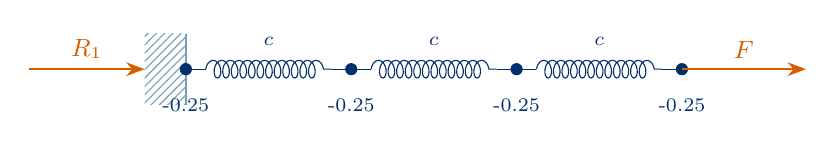
\begin{tikzpicture}[>=Stealth, x=2.1cm, y=1cm]
    \fill[pattern=north east lines, pattern color=fautech] (-0.25,-0.45) rectangle (0,0.45);
    \draw[fautech, thick] (0,-0.45) -- (0,0.45);
    \foreach \k in {0,1,2} {
      \draw[faublue, decorate, decoration={coil, aspect=0.6, segment length=3.1pt, amplitude=3.2pt}]
        (\k+0.12,0) -- (\k+0.88,0);
      \draw[faublue] (\k,0) -- (\k+0.12,0);
      \draw[faublue] (\k+0.88,0) -- (\k+1,0);
      \node[faublue, font=\scriptsize, above] at (\k+0.5,0.18) {$c$};
    }
    \foreach \k in {0,...,3} {
      \fill[faublue] (\k,0) circle (2.2pt);
      \pgfmathparse{int(\k+1)}
      \node[faublue, font=\scriptsize, below] at (\k,-0.25) {\pgfmathresult};
    }
    \draw[->, cs, thick] (3,0) -- (3.75,0) node[above, midway, font=\small] {$F$};
    \draw[<-, cs, thick] (-0.25,0) -- (-0.95,0) node[above, midway, font=\small] {$R_1$};
  \end{tikzpicture}
  \caption{Chain of three massless springs of stiffness $c$ between four nodes, clamped at
    node~1 and loaded by $F$ at node~4. The reaction $R_1$ is induced by the Dirichlet
    constraint $u_1 = 0$.}
  \label{fig:springs}
\end{figure}

A linear spring between nodes $i$ and $j$ transmits the force $F_{\mathrm{s}} = c\,\Delta u$,
with $\Delta u$ the change of its length. Number the springs by their left node, so that
spring $i$ connects node $i$ to node $i+1$ and carries
\begin{equation}\label{eq:springforce}
  F_i = c\,(u_i - u_{i+1}),
\end{equation}
counted positive when it pulls node $i$ to the right. At every node the forces must
balance. Node 1 carries the reaction $R_1$ and the force of spring 1, node $i$ (interior)
carries the forces of the two springs attached to it with opposite signs, and node 4
carries the external load:
\begin{equation}\label{eq:nodalbalance}
  \begin{aligned}
    \text{node 1:}&\quad R_1 - F_1 = 0, \\
    \text{node 2:}&\quad F_1 - F_2 = 0, \\
    \text{node 3:}&\quad F_2 - F_3 = 0, \\
    \text{node 4:}&\quad F_3 - F = 0.
  \end{aligned}
\end{equation}
Inserting~\eqref{eq:springforce} into each of these gives
\begin{equation}\label{eq:nodalexpanded}
  \begin{aligned}
    R_1 - c\,(u_1 - u_2) &= 0, \\
    c\,(u_1 - u_2) - c\,(u_2 - u_3) &= 0 &&\Longrightarrow&  c\,(-u_1 + 2u_2 - u_3) &= 0,\\
    c\,(u_2 - u_3) - c\,(u_3 - u_4) &= 0 &&\Longrightarrow&  c\,(-u_2 + 2u_3 - u_4) &= 0,\\
    c\,(u_3 - u_4) - F &= 0 &&\Longrightarrow&  c\,(-u_3 + u_4) &= F.
  \end{aligned}
\end{equation}
Collecting the four equations in matrix form, and keeping the reaction on the right-hand
side as a separate vector, yields exactly the system of the script,
\begin{equation}\label{eq:springsystem}
  \boxed{\;
  c\underbrace{\begin{bmatrix}
    1 & -1 & 0 & 0 \\
    -1 & 2 & -1 & 0 \\
    0 & -1 & 2 & -1 \\
    0 & 0 & -1 & 1
  \end{bmatrix}}_{\bK}
  \underbrace{\begin{bmatrix} u_1 \\ u_2 \\ u_3 \\ u_4 \end{bmatrix}}_{\bd}
  = \underbrace{\begin{bmatrix} 0 \\ 0 \\ 0 \\ F \end{bmatrix}}_{\bff}
  - \underbrace{\begin{bmatrix} R_1 \\ 0 \\ 0 \\ 0 \end{bmatrix}}_{\bR}. \;}
\end{equation}
The internal spring forces have cancelled pairwise at every interior node, as they must by
Newton's third law; only the external load and the reaction at the constrained node
survive on the right-hand side.

\subsection{The assembly routine (Task 6.2)}\label{sec:assemblyroutine}

\begin{task}{6.2}
  Implement an assembly routine for linear elements. It should take an element matrix and
  the global numbers of its nodes, and add the element matrix block-wise into the global
  stiffness matrix at the correct positions, so that a loop over all elements fills the
  global matrix.
\end{task}

Comparing~\eqref{eq:springsystem} with the element matrix~\eqref{eq:Ke} shows that the
global matrix of the chain is the sum of three spring matrices, each written into the
$2\times2$ block of rows and columns belonging to its own two nodes. This is the assembly
operation in general: with a connectivity map $k \mapsto (n^k_1, n^k_2)$ from the local to
the global node numbers,
\begin{equation}\label{eq:assembly}
  K_{n^k_a\,n^k_b} \mathrel{+}= K^{e_k}_{ab},
  \qquad a,b \in \{1,\dots,N_{\max}\},
  \qquad k = 1,\dots,n_{\mathrm{el}},
\end{equation}
which in compact notation is written $\bK = \bm{\Lambda}_{k=1}^{n_{\mathrm{el}}}\bK^{e_k}$.
The right-hand side is assembled in the same way; for the Neumann part the ``assembly''
reduces to adding the external forces at the correct global positions, because the internal
contributions at shared nodes cancel as in~\eqref{eq:nodalexpanded}. The accumulation
``$\mathrel{+}=$'' is essential: in one dimension each interior node is shared by two
elements, and its diagonal entry receives $EA/h$ from each of them, giving the $2$ on the
diagonal of~\eqref{eq:springsystem}.

\subsection{Properties of the global stiffness matrix (Task 6.3)}\label{sec:properties}

\begin{task}{6.3}
  Print the assembled global matrix and compare it, for $c = 1$ (or $\bK^e = $ the unit
  spring matrix), with~\eqref{eq:springsystem}. What are the properties of the global
  stiffness matrix? Why can the global system not yet be solved, and what is the physical
  interpretation?
\end{task}

Part~II prints the assembled matrix for three unit springs and verifies entry by entry
that it equals $\bK$ of~\eqref{eq:springsystem}. The matrix has the following properties,
all of which are checked numerically in Part~II.
\begin{enumerate}\setlength{\itemsep}{2pt}
  \item \textbf{Symmetric}, $\bK = \bK^{\mathsf{T}}$. This is inherited from the symmetry
    of each $\bK^e$, which in turn follows from the major symmetry of the stiffness tensor
    (\cref{sec:21}) via the symmetric bilinear form $\bB^{\mathsf{T}}EA\bB$.
  \item \textbf{Sparse and banded.} Two nodes are coupled only if they share an element,
    so in one dimension $\bK$ is tridiagonal with at most three non-zeros per row,
    independent of the number of elements. Assembly never produces a dense matrix.
  \item \textbf{Weakly diagonally dominant with vanishing row sums,}
    $\sum_j K_{ij} = 0$ for every $i$. The row sum is the force produced by a uniform
    translation of the whole mesh.
  \item \textbf{Positive semi-definite.} For any $\bd$,
    $\bd^{\mathsf{T}}\bK\bd = \sum_e \tfrac{EA}{h}(d_{i+1}-d_i)^2 \ge 0$, which is twice
    the stored strain energy and can never be negative.
  \item \textbf{Singular}, with $\operatorname{rank}\bK = n-1$. The null space is spanned
    by the constant vector $\bm{1} = [1,1,\dots,1]^{\mathsf{T}}$, since
    $\bK\bm{1} = \bm{0}$ by property~3.
\end{enumerate}

\paragraph{Why the system cannot be solved, and what that means.}
Because $\bK$ is singular, $\bK\bd = \bff$ has either no solution or infinitely many.
Physically, the assembled system describes a bar (or spring chain) that floats freely in
space: nothing has yet told it where it is. Any solution may be shifted by an arbitrary
rigid-body translation $\alpha\,\bm{1}$ without changing a single strain, hence without
changing any force --- the displacement field is determined only up to that translation, so
no unique solution exists. The same statement read along the rows says that the system is
solvable only if the right-hand side is orthogonal to the null space,
$\bm{1}^{\mathsf{T}}\bff = \sum_i f_i = 0$: the applied forces must themselves be in
equilibrium, otherwise the structure accelerates and the \emph{static} problem has no
solution at all. For the chain of \cref{fig:springs} with $\bff = [0,0,0,F]^{\mathsf{T}}$
this condition is violated, consistent with the fact that the reaction $\bR$ is still
missing. Imposing the Dirichlet condition $u_1 = 0$ removes the rigid-body mode and
supplies the reaction, and makes the reduced matrix positive definite and invertible. That
is the subject of the next section.

% ===============================================================
\section{Dirichlet boundary conditions}\label{sec:dirichlet}
% ===============================================================

\subsection{Reduction by a permutation matrix}\label{sec:reduction}

Split the displacement vector into a known part $\bd_{\Gamma}$, which carries the
prescribed values at the constrained nodes and zeros elsewhere, and the unknown remainder
$\check{\bd}$,
\begin{equation}\label{eq:split}
  \bd = \bd_{\Gamma} + \check{\bd}
  \qquad\Longrightarrow\qquad
  \bK\,\check{\bd} = \bff - \underbrace{\bK\,\bd_{\Gamma}}_{\bR} .
\end{equation}
The product $\bK\bd_{\Gamma}$ is the vector of forces that the prescribed displacements
induce; moving it to the right-hand side is exactly how a non-zero Dirichlet value enters
the load vector. Afterwards the rows and columns of the constrained nodes are deleted. This
can be done directly by slicing, or elegantly by a rectangular permutation (selection)
matrix $\bP \in \R^{(n-m)\times n}$ for $n$ nodes with $m$ constraints, which maps the full
vector to the reduced one,
\begin{equation}\label{eq:permutation}
  \bd_{\mathrm{r}} = \bP\cdot\bd,
  \qquad
  \bP^{\mathsf{T}}\cdot\bd_{\mathrm{r}} = \check{\bd},
  \qquad
  P_{ik}P_{jk} = \delta_{ij}.
\end{equation}
Multiplying~\eqref{eq:split} from the left by $\bP$ and inserting
$\check{\bd} = \bP^{\mathsf{T}}\bd_{\mathrm{r}}$ gives the reduced system and, after the
solve, the reconstruction of the full vector,
\begin{equation}\label{eq:reducedsystem}
  \underbrace{\left(\bP\,\bK\,\bP^{\mathsf{T}}\right)}_{\bK_{\mathrm{r}}}\bd_{\mathrm{r}}
  = \underbrace{\bP\left(\bff - \bK\,\bd_{\Gamma}\right)}_{\bff_{\mathrm{r}}},
  \qquad
  \bd = \bP^{\mathsf{T}}\bd_{\mathrm{r}} + \bd_{\Gamma}.
\end{equation}
Note that $\bP$ is not square and therefore neither orthogonal nor invertible; only the
one-sided relation~\eqref{eq:permutation} holds, and $P_{ki}P_{kj} \ne \delta_{ij}$. Once
at least one node is constrained, $\bK_{\mathrm{r}}$ inherits symmetry and positive
semi-definiteness from $\bK$ but is now \emph{positive definite}: a non-zero
$\bd_{\mathrm{r}}$ cannot be a rigid-body translation, because the constrained node is held
at zero, so some element must be strained and the energy is strictly positive. Hence
$\bK_{\mathrm{r}}$ is invertible and the Cholesky solver of \cref{sec:oneelement} applies.

\subsection{The permutation matrix for a $4\times4$ system (Task 7.1)}\label{sec:permutation}

\begin{task}{7.1}
  Write down by hand the permutation matrix for a $4\times4$ system with a Dirichlet
  boundary condition acting on the first node.
\end{task}

With $n = 4$ nodes and $m = 1$ constraint on node~1, the reduced vector contains the
displacements of nodes 2, 3, 4, and $\bP$ has the dimension
$(n-m)\times n = 3\times 4$. Each row selects one surviving node:
\begin{equation}\label{eq:P}
  \boxed{\;
  \bP = \begin{bmatrix}
    0 & 1 & 0 & 0 \\
    0 & 0 & 1 & 0 \\
    0 & 0 & 0 & 1
  \end{bmatrix},
  \qquad
  \bd_{\mathrm{r}} = \bP\,\bd = \begin{bmatrix} u_2 \\ u_3 \\ u_4 \end{bmatrix}. \;}
\end{equation}
Applying it to the spring system~\eqref{eq:springsystem} with $u_1 = 0$ gives
\begin{equation}\label{eq:springreduced}
  \bK_{\mathrm{r}} = \bP\,\bK\,\bP^{\mathsf{T}}
  = c\begin{bmatrix}
    2 & -1 & 0 \\
    -1 & 2 & -1 \\
    0 & -1 & 1
  \end{bmatrix},
  \qquad
  \bff_{\mathrm{r}} = \begin{bmatrix} 0 \\ 0 \\ F \end{bmatrix},
\end{equation}
which is exactly eq.~(54) of the script. This matrix is non-singular
($\det\bK_{\mathrm{r}} = c^3 > 0$) and its solution is
$\bd_{\mathrm{r}} = (F/c)\,[1,2,3]^{\mathsf{T}}$: each spring is stretched by the same
amount $F/c$, so the displacement grows linearly along the chain, the discrete analogue of
$u(x) = Fx/(EA)$.

\subsection{Non-zero prescribed displacements (Task 7.2)}\label{sec:nonzero}

\begin{task}{7.2}
  Program a scheme that modifies the global system for Dirichlet boundary conditions,
  taking the node number and the prescribed displacement as input. Be careful with
  non-zero values. Test it on the spring system with $u_1 = 0$, and in a second case
  replace the Neumann condition by a second, non-zero Dirichlet condition $u_4 \ne 0$.
\end{task}

The subtlety with non-zero values is the term $\bK\bd_{\Gamma}$ in~\eqref{eq:split}, which
is often forgotten: simply deleting rows and columns is correct only for homogeneous
conditions. For the second test case, $u_1 = 0$ and $u_4 = \bar{u} \ne 0$ with no external
force, $n - m = 2$ unknowns remain and the right-hand side becomes
\begin{equation}\label{eq:rhs-nonzero}
  \bff - \bK\,\bd_{\Gamma}
  = \bm{0} - c\begin{bmatrix}
    1 & -1 & 0 & 0 \\ -1 & 2 & -1 & 0 \\ 0 & -1 & 2 & -1 \\ 0 & 0 & -1 & 1
  \end{bmatrix}
  \begin{bmatrix} 0 \\ 0 \\ 0 \\ \bar{u} \end{bmatrix}
  = c\begin{bmatrix} 0 \\ 0 \\ \bar{u} \\ -\bar{u}\end{bmatrix},
\end{equation}
so the reduced system for $[u_2, u_3]^{\mathsf{T}}$ reads
\begin{equation}\label{eq:reduced-nonzero}
  c\begin{bmatrix} 2 & -1 \\ -1 & 2 \end{bmatrix}
  \begin{bmatrix} u_2 \\ u_3 \end{bmatrix}
  = c\begin{bmatrix} 0 \\ \bar{u} \end{bmatrix}
  \qquad\Longrightarrow\qquad
  u_2 = \frac{\bar{u}}{3},
  \quad u_3 = \frac{2\bar{u}}{3},
\end{equation}
the expected uniform stretch of all three springs. Part~II reproduces both test cases and
additionally checks that the reaction forces recovered from the deleted rows sum to zero.

% ===============================================================
\section{Results of the finite element analysis}\label{sec:results}
% ===============================================================

\begin{task}{8.1}
  Perform a linear one-dimensional finite element analysis of the problem of Task~2.3 with
  $n = 6$ elements using all the subroutines developed above, compute the approximate
  stress field, plot the results, and investigate different boundary conditions, that is
  several forces and/or prescribed displacements.
\end{task}

\Cref{tab:results} summarizes the results obtained in Part~II; the plots are given there.
The sequence of steps is the one listed in the script: derive the governing equation
(\cref{sec:bar}), formulate the weak form (\cref{sec:weakbar}), discretize
(\cref{sec:shape}), integrate numerically (\cref{sec:quadrature}), assemble
(\cref{sec:assembly}), impose boundary conditions (\cref{sec:dirichlet}), solve, and
post-process the stress as $\tilde\sigma = E\,\bB\cdot\buh$ on each element.

\begin{table}[ht]
  \centering
  \caption{Summary of the numerical results of Part~II for the bar of Task~2.3
    ($E = \num{210000}\,\mathrm{N/mm^2}$, $A = 25\,\mathrm{mm^2}$, $l = 50\,\mathrm{mm}$,
    $F = 5\,\mathrm{N}$).}
  \label{tab:results}
  \begin{tabularx}{\linewidth}{lXl}
    \toprule
    Case & Result & Error \\
    \midrule
    1 element, $u_1 = 0$, $F$ at node 2
      & $\hat u_2 = \num{4.7619e-5}\,\mathrm{mm}$, $\sigma = 0.2\,\mathrm{N/mm^2}$
      & $<10^{-16}$ rel. \\
    6 elements, $u_1 = 0$, $F$ at node 7
      & $u$ linear, $\sigma = 0.2\,\mathrm{N/mm^2}$ on every element
      & $<10^{-15}$ rel. \\
    6 elements, two forces
      & piecewise linear $u$, piecewise constant $\sigma$ with a jump at the loaded node
      & exact \\
    6 elements, $u_1 = 0$, $u_7 = \bar u$
      & uniform stretch, $\sigma = E\bar u/l$, reactions $\mp EA\bar u/l$
      & exact \\
    Tapered bar, $A(x)$ linear
      & $\bigO{h^2}$ convergence of the displacement, $\bigO{h}$ of the stress
      & see Part~II \\
    \bottomrule
  \end{tabularx}
\end{table}

Three observations deserve comment. First, for the constant-section bar without body force
the finite element solution is \emph{exact at every mesh size}, for the reason given in
\cref{sec:oneelement}: the exact solution lies in the finite element space. Refinement is
pointless for this particular problem and the six-element run of Task~8.1 serves to verify
the code, not to improve the answer. Second, as soon as the problem leaves that space ---
by giving the bar a varying cross-section $A(x)$ or switching on a body force --- the
expected convergence rates appear, $\bigO{h^2}$ in the displacement and $\bigO{h}$ in the
stress, the latter being one order lower because the stress involves a derivative of the
interpolant. Third, the piecewise constant stress field is discontinuous across element
boundaries whenever the exact stress varies; this is a well-known artefact of
$C^0$-continuous elements and motivates the stress smoothing and superconvergent patch
recovery used in production codes.

% ===============================================================
\section{Conclusion}\label{sec:conclusion}
% ===============================================================

Starting from Newton's second law we derived the local balance of linear momentum and its
static form, used the symmetry of the stress and strain tensors and the existence of a
strain energy density to reduce the stiffness tensor from $81$ through $36$ to $21$
independent components, and specialized the three-dimensional theory to a clamped bar,
obtaining $\mathrm{d}(EA\,u')/\mathrm{d}x + A\rho b = 0$. Multiplying by a test function
that vanishes on the Dirichlet boundary and integrating by parts produced the weak form, in
which the Neumann condition appears naturally and the differentiability requirement on $u$
drops to one derivative.

The discretization used linear Lagrange shape functions, which reproduce exactly the
polynomials of degree at most one and therefore give a piecewise constant strain and
stress field. We showed that the $n$-point closed Newton--Cotes rule is exact for
polynomials of degree $n-1$, and of degree $n$ for odd $n$ by a symmetry argument, so that
the trapezoidal rule integrates the linear-element stiffness exactly, while quadratic
elements require Simpson's rule. Evaluating the element integrals gave the familiar
$\bK^e = (EA/h)\,[[1,-1],[-1,1]]$, formally identical to a linear spring, and assembly by
accumulation into the global node positions produced a symmetric, tridiagonal, positive
semi-definite but singular global matrix whose null space is the rigid-body translation.
Imposing one Dirichlet condition --- by deleting rows and columns, or equivalently by the
rectangular permutation matrix~\eqref{eq:P} --- removes that mode, makes the reduced matrix
positive definite, and allows a Cholesky solve. Solved by hand for a single element, the
system gives $\hat u_2 = F l/(EA) = \num{4.7619e-5}\,\mathrm{mm}$, which coincides with the
analytical solution because the exact displacement field is linear and hence contained in
the finite element space. The implementation of all subroutines, their verification against
these hand calculations, the six-element analysis with several sets of boundary conditions,
and the convergence study for a bar with a varying cross-section are reported in Part~II.

% ===============================================================
\begin{thebibliography}{99}
% ===============================================================

\bibitem{script}
Institute of Materials Simulation (WW8),
``Solid mechanics and linear finite element analysis,''
Materials Simulation Practical No.~2, tutorial script,
Friedrich-Alexander-Universit\"at Erlangen-N\"urnberg.

\bibitem{zienkiewicz2013}
O.~C.~Zienkiewicz, R.~L.~Taylor and J.~Z.~Zhu,
\textit{The Finite Element Method: Its Basis and Fundamentals},
7th~ed.,
Butterworth-Heinemann, Oxford, 2013.

\bibitem{hughes2000}
T.~J.~R.~Hughes,
\textit{The Finite Element Method: Linear Static and Dynamic Finite Element Analysis},
Dover, Mineola, NY, 2000.

\bibitem{belytschko2014}
T.~Belytschko, W.~K.~Liu, B.~Moran and K.~I.~Elkhodary,
\textit{Nonlinear Finite Elements for Continua and Structures},
2nd~ed.,
Wiley, Chichester, 2014.

\bibitem{holzapfel2000}
G.~A.~Holzapfel,
\textit{Nonlinear Solid Mechanics: A Continuum Approach for Engineering},
Wiley, Chichester, 2000.

\bibitem{gurtin2010}
M.~E.~Gurtin, E.~Fried and L.~Anand,
\textit{The Mechanics and Thermodynamics of Continua},
Cambridge University Press, Cambridge, 2010.

\bibitem{nye1985}
J.~F.~Nye,
\textit{Physical Properties of Crystals: Their Representation by Tensors and Matrices},
Oxford University Press, Oxford, 1985.

\bibitem{stoer2002}
J.~Stoer and R.~Bulirsch,
\textit{Introduction to Numerical Analysis},
3rd~ed.,
Springer, New York, 2002.

\bibitem{golub2013}
G.~H.~Golub and C.~F.~Van~Loan,
\textit{Matrix Computations},
4th~ed.,
Johns Hopkins University Press, Baltimore, MD, 2013.

\bibitem{braess2007}
D.~Braess,
\textit{Finite Elements: Theory, Fast Solvers, and Applications in Solid Mechanics},
3rd~ed.,
Cambridge University Press, Cambridge, 2007.

\end{thebibliography}

\end{document}
